\documentclass[a4paper, zihao=-4, UTF-8]{ctexart}
\usepackage{graphicx}
\usepackage{subfigure}
\usepackage{caption2}

\renewcommand{\figurename}{图}
\renewcommand{\captionlabeldelim}{.}
\renewcommand{\thesubfigure} {\thefigure.\arabic{subfigure}} \makeatletter
\renewcommand{\@thesubfigure}{\thesubfigure:\space} \renewcommand{\p@subfigure}{} \makeatother
\renewcommand{\tablename}{表}

\usepackage{enumerate}

\usepackage {ctex}
\usepackage{hyperref}
\hypersetup{
	colorlinks=true,
	citecolor=black,
	linkcolor=black
}

\usepackage{geometry}
\geometry{a4paper,left=2.5cm,right=2.5cm,top=2.5cm,bottom=2.5cm}
\setlength{\parindent}{2em}
\setmonofont{Consolas}
\setsansfont{Consolas}
\setmainfont{Times New Roman}

\usepackage{fancyhdr}
\pagestyle{fancy}
\renewcommand{\headrulewidth}{0pt}

\usepackage{authblk}
\renewcommand*{\Affilfont}{\small} % 修改机构名称的字体与大小
\renewcommand\Authand{, } % 去掉 and 前的逗号

\usepackage{indentfirst}
\setlength{\parindent}{2em}

\usepackage{amsmath}
\usepackage{amssymb}
\CTEXsetup[format={\Large\bfseries}]{section}
\usepackage{xcolor}
\usepackage{listings}
\renewcommand{\lstlistingname}{代码}
\lstset{
	columns=fixed,
	breakatwhitespace=true,
	breaklines=true,
	breakindent=26pt,
	captionpos=bl,
	numbers=left,
	frame=shadowbox,
	basicstyle=\ttfamily,
	keywordstyle=\ttfamily\color{blue},
	numberstyle=\footnotesize\color{darkgray},
	commentstyle=\ttfamily\it\color[RGB]{0,96,96},
	stringstyle=\ttfamily\color{magenta},
	showstringspaces=false,
	language=Python,
	identifierstyle=\ttfamily,
	tabsize=4,
}

\usepackage{algorithm}
\usepackage{algorithmicx}
\usepackage{algpseudocode}
\renewcommand{\algorithmicrequire}{\textbf{Input:}}  % Use Input in the format of Algorithm  
\renewcommand{\algorithmicensure}{\textbf{Output:}} % Use Output in the format of Algorithm  

\usepackage{appendix}
\renewcommand{\appendixname}{Appendix~\Alph{section}}
\usepackage{cleveref}
\crefname{equation}{式}{式}
\crefname{figure}{图}{图}
\crefname{table}{表}{表}
\crefname{appendix}{附录}{附录}
\crefname{algorithm}{算法}{算法}
\crefname{listing}{代码}{代码}
\newcommand{\crefpairconjunction}{~和~}
\newcommand{\crefmiddleconjunction}{、}
\newcommand{\creflastconjunction}{~和~}
\newcommand{\crefpairgroupconjunction}{~和~}
\newcommand{\crefmiddlegroupconjunction}{、}
\newcommand{\creflastgroupconjunction}{~和~}
\newcommand{\crefrangeconjunction}{~到~}

\usepackage{cite}
\newcommand{\upcite}[1]{{\textsuperscript{\cite{#1}}}}

\title{\textbf{密码学实验第七次实验报告} }
\date{}
\begin{document}
	\maketitle
	\tableofcontents
	\newpage
	\section{实验目的}
	\begin{enumerate}[1.]
		\item 了解常用的流密码算法,并对其进行实现;
		\item 了解常用的伪随机数生成算法,并对其进行实现。
	\end{enumerate}
	\section{实验原理}
		流密码(Stream Cipher)也成为序列密码,它是对称密码算法的一种。流密码具有实现简单、便于硬件实施、加解密处理速度快、没有或只有有限的错误传播等特点,因此在实际应用中,特别是专用或机密机构中保持着优势,典型的应用领域包括无线通信、外交通信。
	\section{实验环境}
	\paragraph*{系统环境} Windows10 WSL Ubuntu20.04。
	\paragraph*{运行环境} Python3.6与Python3.7。
	\section{实验内容}
		\subsection{BBS伪随机数生成器}
			\subsubsection{算法原理}
				BBS(Blum  Blum Shub)是一种伪随机数生成器,其生成的随机数结果取决于一个随机种子。BBS的产生过程如下:
				\begin{enumerate}[1.]
					\item 选择两个大素数$p, q$,且有$p\equiv q\equiv 3\pmod 4$,令$n=p\times q$,
					\item 选择一个随机数$s$,要求$\gcd(s, n)=1$,
					\item 通过$X_{i+1}=X_i^2\mod n, B_i=X_i\mod 2$生成位$B_i$序列。
				\end{enumerate}
				
				由于大数的分解是困难的,对于给定的$n$,无法确定其因子$p, q$,因此对于给定的最初$k$位序列,都无法以超过$\dfrac{1}{2}$的概率预测出下一位是$0$还是$1$。
			\subsubsection{算法流程}
				BBS伪随机数生成器的流程图如\cref{fig:round_crypt_flow_chart}所示。
				\begin{figure}[htbp]
					\centering
					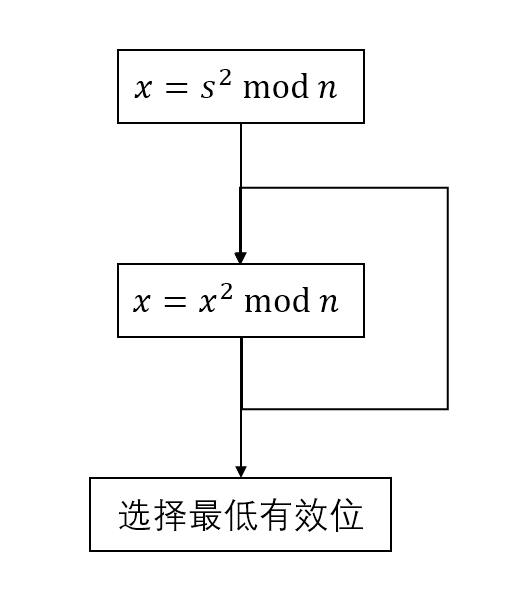
\includegraphics[width=0.6\textwidth]{BBS流程图.png}
					\caption{BBS算法流程图}
					\label{fig:round_crypt_flow_chart}
				\end{figure}
			
				BBS伪随机数生成算法的伪代码如\cref{alg:blum_blum_shub}所示。
				
				\begin{algorithm}[htbp]
					\caption{BBS随机数生成器}
					\label{alg:blum_blum_shub}
					\begin{algorithmic}[1]
						\Require $\mathrm{Big\ prime}: p, q, \mathrm{Seed}:s, \mathrm{Number}:num$
						\Ensure $\mathrm{Pseudorandom\ number}: B$
						\Function{BBS}{$p, q, s, num$}
						\State $n \gets p \times q$;
						\State $X \gets s^2 \mod n$;
						\State $B \gets X \& 1$;
						\For{$i = 1 \to num$}
							\State $X \gets X^2\mod n$;
							\State $B \gets (B \ll 1) | (X \& 1)$;
						\EndFor
						\State \Return{$B$}
						\EndFunction
					\end{algorithmic}
				\end{algorithm}
			
			\subsubsection{测试样例及结果截图}
				BBS实验测试样例采用 $n=p\times q=383\times 503=192649, s = 101355$ 作为输入数据,共生成20bit的伪随机数\upcite{1},其正确结果如\cref{tab:bbstestdata}所示。

				\begin{table}[htbp]
					\centering
					\begin{tabular}{c|c|c|c|c|c}
						\hline
						$i$  &  $X_i$   & $B_i$ & $i$  &  $X_i$   & $B_i$ \\
						\hline
						$0$  & $20749$  &       &      &          &       \\
						\hline
						$1$  & $143135$ & $ 1 $ & $11$ & $137920$ & $ 0 $ \\
						\hline
						$2$  & $177671$ & $ 1 $ & $12$ & $123175$ & $ 1 $ \\
						\hline
						$3$  & $97048$  & $ 0 $ & $13$ & $8630$   & $ 0 $ \\
						\hline
						$4$  & $89992$  & $ 0 $ & $14$ & $114386$ & $ 0 $ \\
						\hline
						$5$  & $174051$ & $ 1 $ & $15$ & $14863$  & $ 1 $ \\
						\hline
						$6$  & $80649$  & $ 1 $ & $16$ & $133015$ & $ 1 $ \\
						\hline
						$7$  & $45663$  & $ 1 $ & $17$ & $106065$ & $ 1 $ \\
						\hline
						$8$  & $69442$  & $ 0 $ & $18$ & $45870 $ & $ 0 $ \\
						\hline
						$9$  & $186894$ & $ 0 $ & $19$ & $137171$ & $ 1 $ \\
						\hline
						$10$ & $177046$ & $ 0 $ & $20$ & $48060$  & $ 0 $ \\
						\hline
					\end{tabular}
					\caption{BBS测试数据}
					\label{tab:bbstestdata}
				\end{table}

				具体的测试代码如\cref{apx:testdata}中的\cref{lst:bbstestdata}所示,由于本次实验较为简单,将测试样例放入源代码文件中。

				其运行结果如\cref{fig:BBS_result}所示。

				\begin{figure}[htbp]
					\centering
					\includegraphics{BBS测试样例结果截图.png}
					\caption{BBS测试样例运行结果}
					\label{fig:BBS_result}
				\end{figure}
				
			
			\subsubsection{总结}
				BBS算法的实现难度较为简单,在具体实现代码中,为了与表格的数据进行对比,确认代码的正确性,函数返回了X和B两个数组。实际实现时,无需存储X和B数组,仅需将所有的B压缩到一个数中即可,十分容易修改。
			
			\subsection{RC4流密码}
				\subsubsection{算法原理}
				RC4由Ron Rivest设计,最初隶属于RSA安全公司。它是一个可变密钥长度,面向字节流的流密码。该算法以随机置换作为基础,实现较为简单,因此广泛应用于SSL/TLS协议和WEP/WPA协议。
				
				RC4算法首先用$1\sim 256$个字节的可变长度密钥初始化一个256字节的数组$S$,$S$中包含$0\sim 255$的所有数字,每个数字均出现且出现一次。对于加密或解密时,字节$k$是从$S$中按照特定方式选择一个元素生成的。每生成一个$k$,$S$就重新置换一次。最后生成的$k$字节流就是密钥流,与明文字节流依次进行异或计算得到密文字节流。
				\subsubsection{算法流程}
				如伪代码\cref{alg:RC4init}所示,初始化$S$部分中,先将$S$按照升序初始化为$0\sim 255$,随后用输入的密钥产生$S$的初始置换,对每个$S[i]$,根据由$K[i]$确定的方案,将$S[i]$与$S$中的另一个字节交换位置。
				\begin{algorithm}[htbp]
					\caption{RC4初始置换}
					\label{alg:RC4init}
					\begin{algorithmic}[1]
						\Require $K$
						\Ensure $S$
						\Function{Init}{$K$}
						\For{$i=0\to 255$}
							\State $S[i]\gets i$;
						\EndFor
						\State $j\gets 0$;
						\For{$i=0\to 255$}
							\State $j\gets(j+S[i]+K[i])\mod 256$;
							\State $\Call{Swap}{S[i], S[j]}$;
						\EndFor
						\State \Return{$S$}
						\EndFunction
					\end{algorithmic}
				\end{algorithm}
			
				RC4的加密与解密通常不单独写为一个函数,而是直接与产生的密钥流进行异或运算,这样无需保存密钥流,节省了大量的空间。当向量$S$初始化完成时,输入的密钥不再使用,而是由当前的$S$生成一个密钥流。其具体过程为:从$S[0]$到$S[255]$,对每个$S[i]$,根据$S$的当前配置,将$S[i]$与$S$中的另一字节替换。当$S[255]$完成置换后,操作将重复从$S[0]$开始。其伪代码如\cref{alg:RC4crypt}所示。
				
				\begin{algorithm}[htbp]
					\caption{RC4初始置换}
					\label{alg:RC4crypt}
					\begin{algorithmic}[1]
						\Require $in, K$
						\Ensure $out$
						\Function{Crypt}{$in, K$}
						\State $S\gets \Call{Init}{K}$;
						\State $i \gets 0$;
						\State $j \gets 0$;
						\State $out\gets \emptyset$
						\ForAll{$m \in in$}
							\State $i\gets (i+1)\mod 256$;
							\State $j\gets (j+S[i])\mod 256$;
							\State $\Call{Swap}{S[i], S[j]}$;
							\State $\Call{Append}{out, m \oplus S[(S[i] + S[j])\mod 256]}$;
						\EndFor
						\State \Return{$out$}
						\EndFunction
					\end{algorithmic}
				\end{algorithm}
			
				\subsubsection{测试样例及结果截图}
					具体的测试代码如\cref{apx:testdata}中的\cref{lst:rc4testdata}所示,由于本次实验较为简单,将测试样例放入源代码文件中。
					
					该测试代码的运行结果如\cref{fig:rc4result}所示
					\begin{figure}[htbp]
						\centering
						\includegraphics{RC4测试样例结果截图.png}
						\caption{RC4测试样例运行结果}
						\label{fig:rc4result}
					\end{figure}
				\subsubsection{总结}
					由于RC4中主要是在进行列表中两个位置数据的交换,因此不适合绘制流程图,以伪代码展示反而更加直观清晰,因此此处仅展示其伪代码。
					
					RC4密码的实现较为简单,加密解密函数完全相同,只需要实现一个即可。这也使得RC4密码的安全性略有不足,将密文输入进行加密,就会返回明文,所以RC4密码不适合单独用于实现加密服务器或者加密硬件,需要与其他密码配合使用。
			\subsection{祖冲之算法}
				\subsubsection{算法原理}
					在2011年,祖冲之密码被批准成为4G国际标准,这是我国商用密码首次走出国门参与国际标准竞争。2012年,国家密码管理局发布正式公告,将祖冲之密码作为中国商用密码算法,其中的祖冲之密码算法(ZUC)用于产生密钥序列。
					
					这个随机数算法可以分为LFSR、BR、F三层。在LFSR层中,采用了$GF(2^{31}-1)$上的16次本原多项式,有着随机性强,周期大的优点。在BR层中,重组的数据具有良好的随机性,且出现的重复概率很小。在非线性函数F中,采用了两个非线性的S盒,因此有良好的非线性、混淆特性和扩散特性。
				\subsubsection{算法流程}
					ZUC算法共分为LFSR、BR、F三层,其函数调用关系图如\cref{fig:zuc-function}所示。
					\begin{figure}[htbp]
						\centering
						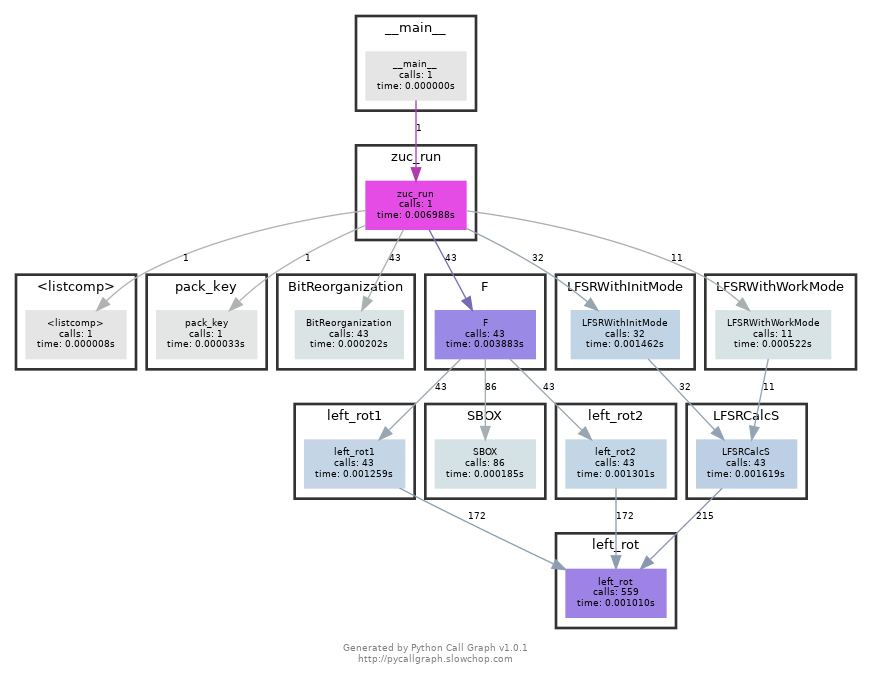
\includegraphics[width=\textwidth]{ZUC函数调用关系图.png}
						\caption{ZUC算法函数调用图}
						\label{fig:zuc-function}
					\end{figure}
					\paragraph{线性反馈移位寄存器}
					线性反馈移位寄存器(LFSR)由16个32位寄存器组成,每一个都是定义在素域$GF(2^{31}-1)$上。LFSR分为两种工作状态,分别是初始化状态和工作状态。其流程图如\cref{fig:ZUC_LFSR_flowchart}所示。
					
					\begin{figure}[htbp]
						\centering
						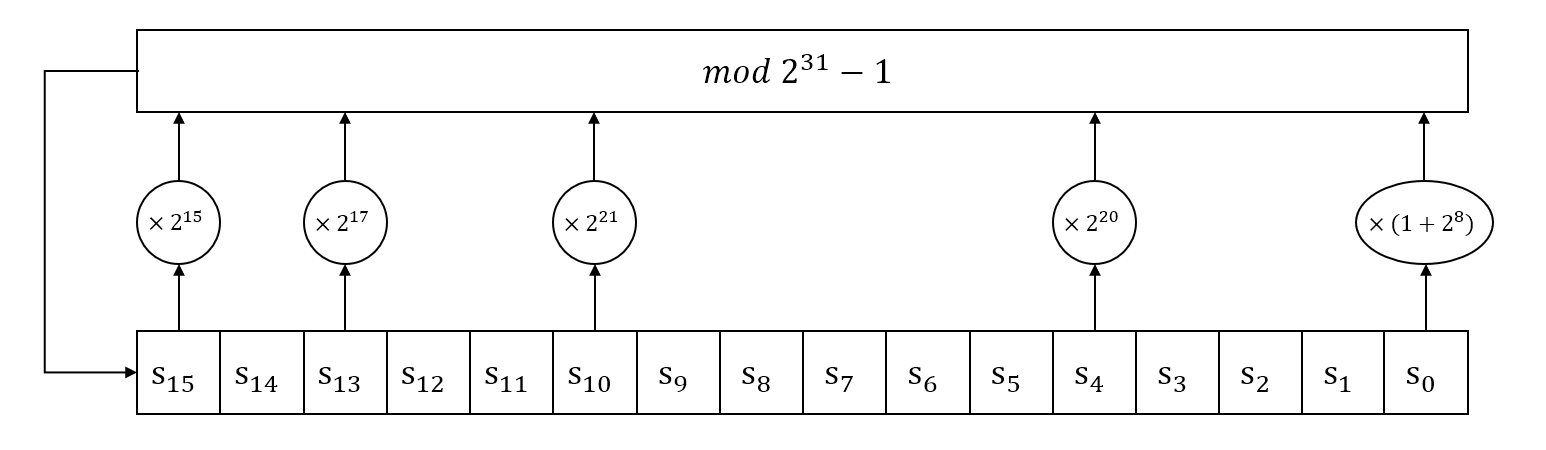
\includegraphics[width=\textwidth]{ZUC流程图LFSR.png}
						\caption{ZUC算法LFSR模式流程图}
						\label{fig:ZUC_LFSR_flowchart}
					\end{figure}
					
					初始化模式的伪代码如所示。工作模式的伪代码如\cref{alg:ZUC_LFSR_Init}所示。由两个模式的伪代码可知,在初始状态中,需要根据输入信息进行寄存器数值的轮运算,作为初始化;而在工作模式中,则无需输入,LFSR根据寄存器中当前结果,进行运算,得到下一个状态。
					
					\begin{algorithm}[htbp]
						\caption{LFSR初始化模式}
						\label{alg:ZUC_LFSR_Init}
						\begin{algorithmic}[1]
							\Require $u$
							\Function{LFSRWithInitialisationMode}{$u$}
							\State $v\gets (2^{15}s_{15}+2^{17}s_{13}+2^{21}s_{10}+2^{20}s_{4}+(1+2^{8})s_{0})\mod(2^{31}-1)$;
							\State $s_{16}\gets v+u\mod (2^{31}-1)$;
							\If{$s_{16} = 0$}
							\State $s_{16}\gets 2^{31}-1$
							\EndIf
							\State $s_0, \ldots, s_{15} \gets s_1, \ldots, s_{16}$;
							\EndFunction
						\end{algorithmic}
					\end{algorithm}
					
					\begin{algorithm}[htbp]
						\caption{LFSR工作模式}
						\label{alg:ZUC_LFSR_Work}
						\begin{algorithmic}[1]
							\Require $u$
							\Function{LFSRWithWorkMode}{$u$}
							\State $s_{16}\gets (2^{15}s_{15}+2^{17}s_{13}+2^{21}s_{10}+2^{20}s_{4}+(1+2^{8})s_{0})\mod(2^{31}-1)$;
							\If{$s_{16} = 0$}
							\State $s_{16}\gets 2^{31}-1$
							\EndIf
							\State $s_0, \ldots, s_{15} \gets s_1, \ldots, s_{16}$;
							\EndFunction
						\end{algorithmic}
					\end{algorithm}
					\paragraph{比特重组}
					比特重组(BR)主要用于进行过渡,从LFSR的8个寄存器中取出128bit的内容组成4个32比特的字,供下层非线性函数F和密钥输出使用。其流程图如\cref{fig:ZUC_BR_flowchart}所示。
					\begin{figure}[htbp]
						\centering
						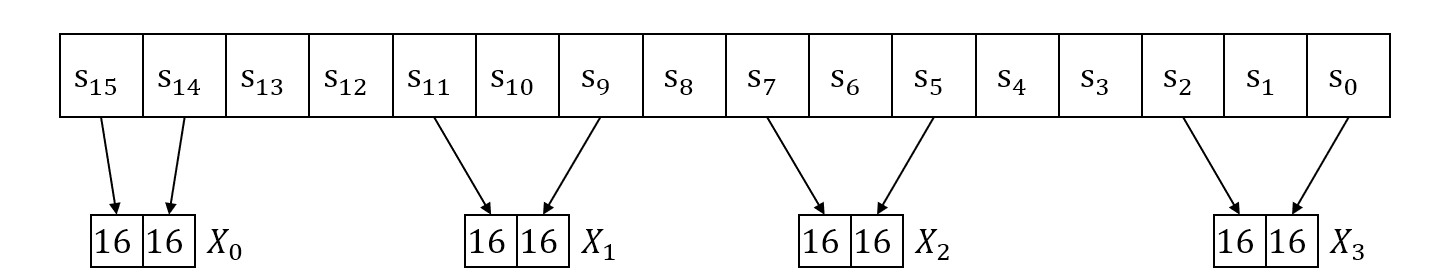
\includegraphics[width=\textwidth]{ZUC流程图BR.png}
						\caption{ZUC算法BR模式流程图}
						\label{fig:ZUC_BR_flowchart}
					\end{figure}
					其伪代码如\cref{alg:ZUC_BR_Work}所示。
					
					\begin{algorithm}[htbp]
						\caption{比特重组BR}
						\label{alg:ZUC_BR_Work}
						\begin{algorithmic}[1]
							\Function{BitReorganization}{}
							\State $X_0\gets s_{15H} \| s_{14L}$;
							\State $X_0\gets s_{11L} \| s_{9H}$;
							\State $X_0\gets s_{7L} \| s_{5H}$;
							\State $X_0\gets s_{2L} \| s_{0H}$;
							\EndFunction
						\end{algorithmic}
					\end{algorithm}
					
					\paragraph{非线性函数}
					非线性函数(F)有两个存储单元$R_1, R_2$,输入为$x_0, x_1, x_2$,输出为32位的$W$。其流程图如\cref{fig:ZUC_F_flowchart}所示。
					\begin{figure}[htbp]
						\centering
						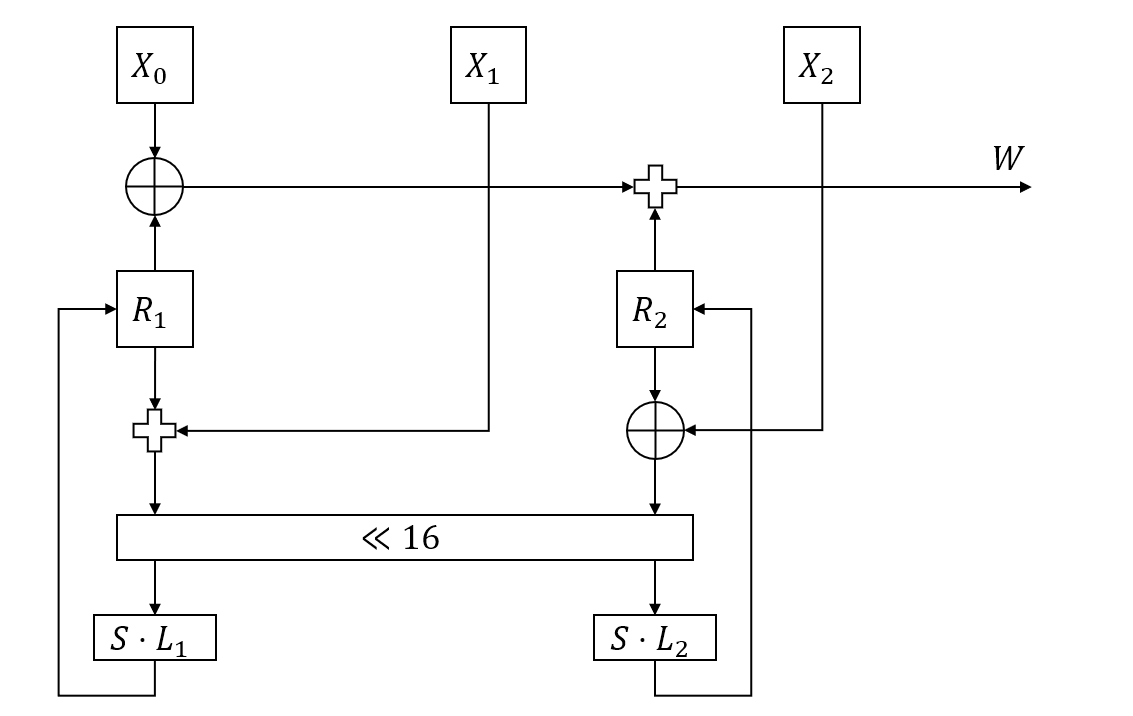
\includegraphics[width=\textwidth]{ZUC流程图F.png}
						\caption{ZUC算法BR模式流程图}
						\label{fig:ZUC_F_flowchart}
					\end{figure}
					伪代码如\cref{alg:ZUC_F_Work}所示。
					
					\begin{algorithm}[htbp]
						\caption{非线性函数F}
						\label{alg:ZUC_F_Work}
						\begin{algorithmic}[1]
							\Require $x_0, x_1, x_2$
							\Ensure $W$
							\Function{F}{$x_0, x_1, x_2$}
							\State $W\gets ((x_0\oplus R_1) + R_2)\mod 2^{32}$;
							\State $W_1\gets (R_1+x_1)\mod 2^{32}$;
							\State $W_2\gets R_2\oplus x_2$;
							\State $t\gets W_{1L}\| W_{2H}$;
							\State $R_1\gets \Call{S}{t\oplus (t\lll_{32}2)\oplus (t\lll_{32}10)\oplus (t\lll_{32}18)\oplus (t\lll_{32}24)}$;
							\State $t\gets W_{2L}\| W_{1H}$;
							\State $R_2\gets \Call{S}{t\oplus (t\lll_{32}8)\oplus (t\lll_{32}14)\oplus (t\lll_{32}22)\oplus (t\lll_{32}30)}$;
							\State \Return{$W$}
							\EndFunction
						\end{algorithmic}
					\end{algorithm}
					
				\subsubsection{测试样例及结果截图}
					具体的测试代码如\cref{apx:testdata}中的\cref{lst:zuctestdata}所示,由于本次实验的数据测试部分较为简单,将测试样例放入源代码文件中。测试结果如\cref{fig:ZUC_result}所示。
					\begin{figure}[htb]
						\centering
						\includegraphics{ZUC测试样例结果截图.png}
						\caption{ZUC测试样例运行结果}
						\label{fig:ZUC_result}
					\end{figure}
				\subsubsection{总结}
					祖冲之算法的具体运行部分只需要按照要求将各个函数进行拼接调用即可,难度较低,因此不进行展开。
					
					祖冲之算法的安全性首先在于其在LFSR层采用了$GF(2^{31})$上的16次本原多项式,输出序列具有随机性好、周期足够大的特点。在非线性函数F中,采用了两个存储部件R、两个线性部分L和两个非线性S盒,输出具有良好的非线性、混淆特性和扩散特性,因此可以抵抗多种密码攻击。其缺点在于,对于测信道攻击,防御效果较差。
		\section{收获与建议}
			本次实验中,为提高代码的可阅读性,将sbox等较大常数均另存于另一个文件中,在当前的python文件使用import调用即可。
			
			此外,由于ZUC需要大量使用全局变量,为了简化难度,没有采用类的方法进行实现,而是将其放入单独的python文件下,开设全局变量,仿照C语言的思路进行实现。
		\begin{thebibliography}{99}
			\bibitem{1}
			(美)William Stallings著. 密码编码学与网络安全——原理与实践(第七版)[M]. 王后珍等译. 北京:电子工业出版社, 2017.
		\end{thebibliography}
		\newpage
		\appendix
			\section{测试样例}\label{apx:testdata}
			\begin{lstlisting}[caption={BBS算法测试样例}, label={lst:bbstestdata}]
from utils import gcd

def BBS(p, q, s, num):
	if(p % 4 != 3 or q % 4 != 3):
		print ("error p, q")
		return 0
	n = p * q
	if (gcd(n, s) != 1):
		print ("error s")
		return 0
	X = [s ** 2 % n]
	B = [X[0] & 1]
	for i in range(num):
		X.append(X[-1] ** 2 % n)
		B.append(X[-1] & 1)
	return X, B

if __name__ == "__main__":
    X, B = BBS(383, 503, 101355, 20)
    for i in range(21):
        print (X[i], B[i])
			\end{lstlisting}
			\begin{lstlisting}[caption={RC4密码测试样例}, label={lst:rc4testdata}]
def __rc4_init(key):
	keylength = len(key)
	S = list(range(256))
	j = 0
	for i in range(256):
		j = (j + S[i] + key[i % keylength]) % 256
		S[i], S[j] = S[j], S[i]
	return S

def rc4_crypt(key, data):
	S = __rc4_init(key)
	i = j = 0
	result = b''
	for a in data:
		i = (i + 1) % 256
		j = (j + S[i]) % 256
		S[i], S[j] = S[j], S[i]
		k = (a ^ S[(S[i] + S[j]) % 256]).to_bytes(1, 'big')
		result += k
	return result

from libnum import n2s, s2n

if __name__ == "__main__":
	X, B = BBS(383, 503, 101355, 20)
	for i in range(21):
	print (X[i], B[i])
	test_rc4 = [
		[0x6e6f742d736f2d72616e646f6d2d6b6579, 0x476f6f6420796f752061726520636f7272656374],
		[0x3475bd76fa040b73f521ffcd9de93f24, 0x1b5e8b0f1bc78d238064826704830cdb],
		[0x2b24424b9fed596659842a4d0b007c61, 0x41b267bc5905f0a3cd691b3ddaee149d],
		[0x0f1571c947d9e8590cb7add6af7f6798, 0x0123456789abcdeffedcba9876543210]
	]
	def convert(k):
		ret = []
		while k > 0:
			ret.append(k & 0xff)
			k >>= 8
		return ret[::-1]
	for test in test_rc4:
		cipher = rc4_crypt(convert(test[0]), convert(test[1]))
		print ('cipher:%x' % int.from_bytes(cipher, 'big', signed = False))
			\end{lstlisting}
			\begin{lstlisting}[caption={ZUC算法测试样例}, label={lst:zuctestdata}]
from ZUC_data import sbox0, sbox1, D

def LFSRCalcS(s):
	return (left_rot(s[15], 15, 31) + left_rot(s[13], 17, 31) + left_rot(s[10], 21, 31) + left_rot(s[4], 20, 31) + left_rot(s[0], 8, 31) + s[0]) % 0x7fffffff

def LFSRWithInitMode(s, u):
	s.append(0x7fffffff if s[0] == 0 else ((LFSRCalcS(s) + u) % 0x7fffffff))
	s.pop(0)

def LFSRWithWorkMode(s):
	s.append(0x7fffffff if s[0] == 0 else LFSRCalcS(s))
	s.pop(0)

def BitReorganization(s):
	X = [0, 0, 0, 0]
	X[0] = ((s[15] & 0x7fff8000) << 1) | (s[14] & 0xffff)
	X[1] = ((s[11] & 0xffff) << 16) | (s[9] >> 15)
	X[2] = ((s[7] & 0xffff) << 16) | (s[5] >> 15)
	X[3] = ((s[2] & 0xffff) << 16) | (s[0] >> 15)
	return X


def left_rot(x, n, x_len):
	return ((x << n) | (x >> (x_len - n))) & ((1 << x_len) - 1)

def left_rot1(x):
	return x ^ left_rot(x, 2, 32) ^ left_rot(x, 10, 32) ^ left_rot(x, 18, 32) ^ left_rot(x, 24, 32)

def left_rot2(x):
	return x ^ left_rot(x, 8, 32) ^ left_rot(x, 14, 32) ^ left_rot(x, 22, 32) ^ left_rot(x, 30, 32)

def SBOX(x):
	return (sbox0[x >> 24] << 24) | (sbox1[(x >> 16) & 0xff] << 16) | (sbox0[(x >> 8) & 0xff] << 8) | (sbox1[x & 0xff])

def F(R, x0, x1, x2):
	W = [0, 0, 0]
	W[0] = ((x0 ^ R[0]) + R[1]) & 0xffffffff
	W[1] = (R[0] + x1) & 0xffffffff
	W[2] = R[1] ^ x2
	R[0] = SBOX(left_rot1((((W[1] & 0xffff) << 16) | (W[2] >> 16))))
	R[1] = SBOX(left_rot2((((W[2] & 0xffff) << 16) | (W[1] >> 16))))
	return W[0]

def pack_key(s, k, iv):
	for i in range(15, -1, -1):
	s[i] = ((k & 0xff) << 23) | (D[i] << 8) | (iv & 0xff)
	k >>= 8
	iv >>= 8

def zuc_run(k, iv, key_len):
	s = [0 for i in range(16)]
	R = [0, 0]
	# init mode
	pack_key(s, k, iv)
	for i in range(32):
		X = BitReorganization(s)
	W = F(R, X[0], X[1], X[2])
	LFSRWithInitMode(s, W >> 1)
	# work mode
	X = BitReorganization(s)
	F(R, X[0], X[1], X[2])
	LFSRWithWorkMode(s)
	Z = []
	for i in range(key_len):
		X = BitReorganization(s)
		Z.append(F(R, X[0], X[1], X[2]) ^ X[3])
		LFSRWithWorkMode(s)
	return Z

if __name__ == '__main__':
	a = zuc_run(0, 0, 2)
	print ('%x\n%x\n' % (a[0], a[1]))
	a = zuc_run(0xffffffffffffffffffffffffffffffff, 0xffffffffffffffffffffffffffffffff, 2)
	print ('%x\n%x\n' % (a[0], a[1]))
	a = zuc_run(0x3d4c4be96a82fdaeb58f641db17b455b, 0x84319aa8de6915ca1f6bda6bfbd8c766, 2)
	print ('%x\n%x\n' % (a[0], a[1]))
	a = zuc_run(0x338985fedc98cb99c9f9b346bd6cae56, 0x7dd3175c2374c7113bcbbfb339563172, 10)
	for a_i in a:
		print ('%x' % (a_i))
			\end{lstlisting}
\end{document}